\documentclass[12pt]{article}

\usepackage[top=3.5cm, bottom=3cm, left=2.5cm , right=2.5cm]{geometry}

\usepackage[utf8]{inputenc}
\usepackage[T1]{fontenc}
\usepackage[francais]{babel}
\usepackage{hyperref}
\usepackage{amsfonts}
\usepackage{amsmath}
\usepackage{amssymb}
\usepackage{setspace}
\usepackage{fancyhdr}
\usepackage{lipsum}
\usepackage{graphicx}

\newcommand{\Matiere}{Génie des Logiciels et des Systèmes}
\newcommand{\titre}{Modèles de Processus}

\title{\Matiere:\\ \titre}
\author{Thibault MEUNIER \and Matthieu PERRIER}
\date{28 octobre 2016}

\pagestyle{fancy}
\lhead{\Matiere}
\rhead{\titre}
\rfoot{Page \thepage}
\cfoot{}
\lfoot{ENSEEIHT - IMA 2A}

\begin{document}
\maketitle

\setcounter{page}{0}
\thispagestyle{empty} % enlever numerotation de la page

\newpage

\section*{Introdution}
L'objectif de ce BE est de mettre en place une nouvelle représentation de processus appelé simplePDL. L'utilisateur devra pouvoir éditer des processus rapidement et graphiquement, tout en vérifiant que les contraintes soient vérifiées.
Pour cette vérification, on utilisera l'outil TINA, qui travaille sur des réseaux de Pétri, d'où le besoin de créer des outils de conversion de modèle à modàle, et de modèle à texte.


\renewcommand{\contentsname}{Sommaire}
\setcounter{tocdepth}{2}
\tableofcontents
\newpage

\section{Les modèles simplePDL et PetriNet et leurs contraintes}
\subsection{Modèle PetriNet}
\subsubsection{Présentation}
Un réseau de Pétri est un modèle permettant de modéliser et de vérifier le comportement de systèmes à événements discrets. Il est composé de places et de transitions reliées entre elles par de arcs. La Figure~\ref{fig:PetriNet} représente la modélisation que nous avons implanté.
\begin{figure}[!h]
  \centering
  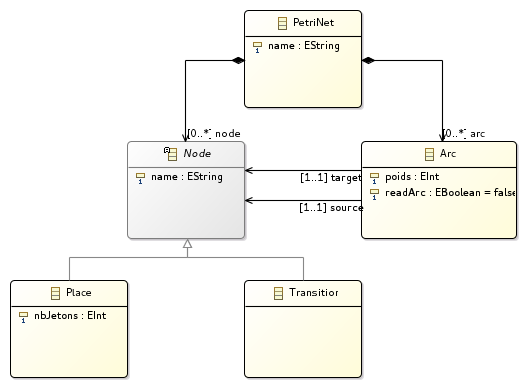
\includegraphics[width=0.7\textwidth]{PetriNet.png}
  \caption{Diagramme du métamodèle PetriNet}\label{fig:PetriNet} 
\end{figure}

\subsubsection{Contraintes}
Un tel model permet la construction de modèles invcalides. Par exemple, on pourrait lier deux places avec un arc. Pour obtenir un modèle conforme au métamodèle réseau de Pétri, il a fallu le compléter avec les contraintes suivantes en OCL :
\paragraph*{Contraintes sur les arcs :}
\begin{description}
\item[sourceTypeDiffTarget] Un arc ne peut pas relier deux n\oe uds de même type.
\item[positive] Un arc a un poid strictement positif
\end{description}

\paragraph*{Contraintes sur les n\oe uds}
\begin{description}
\item[positive] Un n\oe ud contient un nombre positif ou nul de jetons
\end{description}

\subsection{Modèle simplePDL}
\subsubsection{Présentation}
SimplePDL est un métamodèle de représentation de processus. Il défini le concept de processus (\textsf{Process}) composé d'activités (\textsf{WorkDefinition}) qui peuvent dépendre les une sur les autres (\textsf{WorkSequence}). Il définit également le concept de ressources (\textsf{Ressource}) et de leur consommations par les activités (\textsf{RessourceSequence}). Pour finir, on peut ajouter un commentaire (\textsf{Guidance} concernant une activité. La Figure~\ref{fig:simplePDL} représente la modélisation que nous avons implanté.
\begin{figure}[!h]
  \centering
  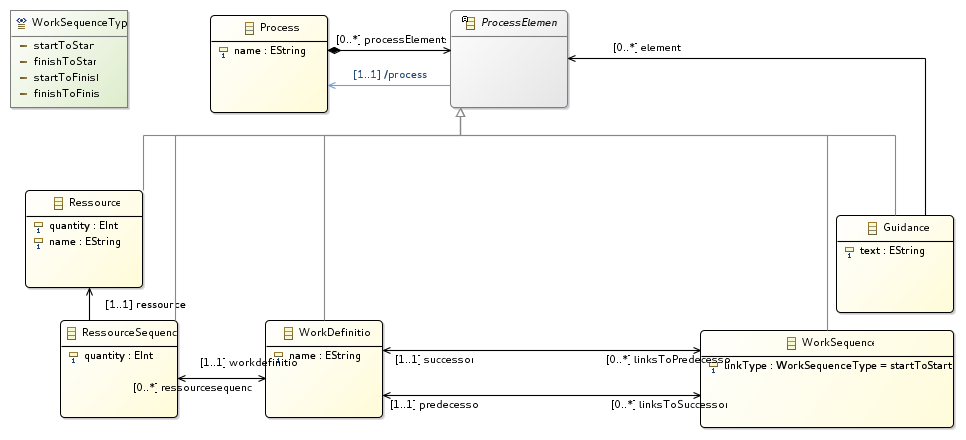
\includegraphics[width=1\textwidth]{simplePDL.png}
  \caption{Diagramme du métamodèle simplePDL}\label{fig:simplePDL} 
\end{figure}

\subsubsection{Contraintes}
Ici encore, il faut rajouter les contraintes OCL suivantes pour obtenir un modèle conforme au métamodèle.
\paragraph*{Contraintes sur Process :}
\begin{description}
\item[nameForbidden] Un Processus ne peut pas s'appeler 'Process'.
\item[differentNames] Deux processus ne peuvent pas avoir le même nom.
\end{description}

\paragraph*{Contraintes sur WorkDefinition :}
\begin{description}
\item[nameNotEmpty] Le nom d'un WorkDefinition n'est pas vide.
\end{description}

\paragraph*{Contraintes sur WorkSequence :}
\begin{description}
\item[previousWDinSameProcess] La Work sequence et sa WorkDefinition source sont dans le même processus.
\item[nextWDinSameProcess] Idem avec la WorkDefinition cible.
\item[notReflexive] Une WorkSequence ne boucle pas sur la même 
WorkDefinition.
\end{description}

\paragraph*{Contraintes sur Ressource :}
\begin{description}
\item[nameNotEmpty] Le nom d'un WorkDefinition n'est pas vide.
\item[quantityPositive] Il y a au moins une instance de cette ressource.
\end{description}

\paragraph*{Contraintes sur RessourceSequence :}
\begin{description}
\item[quantityPositive] Il faut au moins une instance de la ressource.
\item[quantityAvailable] Il existe assez d'instance de la ressource.
\end{description}

\section{Transformations de modèle}
\subsection{Transformation de modèle à modèle}
\subsubsection{SimplePDL to PetriNet}
Un \textsf{Process} peut être transformé en un \textsf{PetriNet}. Pour cela, chaque \textsf{WorkDefinition} peut être modélisée en un ensemble de places et transition comme schématisé sur la Figure~\ref{fig:WDPetriNet}. Puis, chaque \textsf{WorkSequence} correspond à un read-arc entre les n\oe uds appropriés. Enfin, une \textsf{Ressource} est une place et une \textsf{RessourceSequence} correspond à deux arcs : un pour la consommation et un pour la restitution des ressources.

\begin{figure}[!h]
  \centering
  \includegraphics[width=0.2\textwidth]{WDPetriNet.pdf}
  \caption{Diagramme du métamodèle PetriNet}\label{fig:WDPetriNet} 
\end{figure}

Cette transformation à été implanté en Java, puis en ATL.

\subsection{Transformation de modèle à texte}
Quatre transformation de modèle à texte ont été implantés :
\begin{itemize}
\item PetriNet to dot
\item PetriNet to TINA
\item SimplePDL to dot
\item SimplePDL to LTL
\end{itemize}

Ces transformations ont été implémentées en utilisant le language ATL. La mixité avec OCL n'a pas rendu cette transformation aisée, la syntaxe obtenue n'étant pas très lisible.

\subsection{Transformation de texte à modèle}
Il est nécessaire de définir une manière textelle de modélistaion des languages, afin de pouvoir rapidemment vérifier et importer une modélisation. Ainsi, le language textuel défini se doit concis et lisible. XText fourni des outils d'analyse textuels puissants intégrés à Eclipse. 
La principale difficultée a été la modélisation du language et les différents liens dynamiques entre les éléments.

\section{L'éditeur graphique Sirius}
Nous avons utilisé l'éditeur graphique Sirius pour pouvoir modifier des processus modélisés en SimplePDL graphiquement. Il y a la possibilité d'ajouter dynamiquement tous les éléments modélisés. 
La principale difficultées rencontrée lors de cette étape a été d'implanter une coloration conditionelle des fleches représentant les WorkSequences en fonction de leur type. En effet, la syntaxe n'est pas évidente et non décrite dans les TPs.
La Figure~\ref{fig:Conception} montre la vue obtenue pour le process Developpement.
\begin{figure}[!h]
  \centering
  \includegraphics[width=0.7\textwidth]{Conception.png}
  \caption{Représentation du process Develeppement dans l'éditeur graphique}\label{fig:Conception} 
\end{figure}
\newpage

\section{Exemples et tests}
Nous avons essayer de tester tous les invariants de nos modèles séparémment, puis nous avons tester le tout avec des exemple correct le plus concrets et distincts possible.


\end{document}